\documentclass[11pt]{article}

\usepackage[margin=1in]{geometry}
\usepackage{amsmath,amssymb,mathtools,bm}
\usepackage{graphicx}
\usepackage{booktabs,longtable,array,multirow}
\usepackage{enumitem}
\usepackage{xcolor}
\usepackage{microtype}
\usepackage{caption,subcaption}
\usepackage{float}
\usepackage{listings}
\usepackage{hyperref}
\usepackage[nameinlink,noabbrev]{cleveref}

\graphicspath{{figures/}}
\hypersetup{
  colorlinks=true,
  linkcolor=blue!55!black,
  citecolor=green!35!black,
  urlcolor=blue!60!black,
  pdftitle={From 2D GCNM to Peripheral Vascular Impedance Imaging},
}

\definecolor{inblue}{HTML}{4C78A8}
\definecolor{pviorange}{HTML}{F58518}
\definecolor{resultred}{HTML}{E45756}
\definecolor{lightgray}{HTML}{F4F4F4}

\newcommand{\R}{\mathbb{R}}
\newcommand{\E}{\mathbb{E}}
\newcommand{\norm}[1]{\left\lVert #1\right\rVert}
\newcommand{\trans}{^{\mathsf T}}
\newcommand{\sig}{\bm{\sigma}}
\newcommand{\dv}{\Delta\bm{v}}
\newcommand{\dsig}{\Delta\bm{\sigma}}
\newcolumntype{L}[1]{>{\raggedright\arraybackslash}p{#1}}
\newcommand{\plain}[1]{%
  \begin{quote}\color{blue!45!black}\textbf{Engineering interpretation.} #1\end{quote}}

\lstset{
  basicstyle=\ttfamily\small,
  backgroundcolor=\color{lightgray},
  frame=single,
  breaklines=true,
  columns=fullflexible,
}

\title{\textbf{From 2D Graph-Convolutional Newton Methods to\\
Peripheral Vascular Impedance Imaging}\\[0.5em]
\large Original Injun Lee implementation, implemented nonlinear PVI adaptation,
mathematical derivation, experiments, results, and validation roadmap}
\author{Technical project report}
\date{12 July 2026}

\begin{document}
\maketitle

\begin{abstract}
Electrical impedance tomography (EIT) seeks an interior conductivity field from
boundary-current and boundary-voltage measurements.  The problem is nonlinear,
ill-conditioned, and severely underdetermined.  Injun Lee's original two-dimensional
Graph-Convolutional Newton Method (GCNM) combines a Levenberg--Marquardt (LM) update
with a graph convolutional network (GCN) on the finite-element mesh.  At every
learned stage, the original code recomputes the nonlinear forward solution and
Jacobian at the current conductivity estimate; a new stage-specific GCN then maps
the current estimate and LM update directly to the clean conductivity target.

This report derives that method from the complete electrode model, audits the
original code step by step, and compares it with our adaptation for an eight-electrode
peripheral vascular impedance (PVI) ring.  Our PVI system has only 32 measurements
per frame, compared with 928 in the original 32-electrode PyEIT protocol.  We
established production-pipeline parity for subject 6 and the US120 ring, constructed
matched 5,320-element forward and 1,330-element inverse meshes, and trained on clean
synthetic vascular conductivity changes rather than PVI images.  The earlier
fixed-feature experiment improved nonlinear-holdout image correlation from 0.265
(Newton) to 0.463, but increased background energy and image root-mean-square error
(RMSE).  We therefore implemented the defining GCNM mechanism: every learned stage
now recomputes the PVI forward solution, nonlinear residual, Jacobian, and LM
proposal.  On 32 exact nonlinear fine-mesh holdout phantoms, the selected deployable
homogeneous-baseline model reaches image correlation 0.557, image RMSE 0.00432,
Dice 0.485, and background RMS 0.00128; the matched two-step LM-only control reaches
correlation 0.291.  Real subject-6 outputs are evaluated separately against archived
PVI pseudo-reconstructions because paired anatomical conductivity truth is absent.
\end{abstract}

\tableofcontents
\newpage

\section{Purpose, audience, and principal conclusion}

This document is written for two audiences simultaneously.  A telecommunications
graduate should be able to follow the signal model, inverse problem, and algorithmic
flow without prior EIT specialization.  A doctoral reader should find explicit
model assumptions, weak forms, normal equations, identifiability arguments,
implementation distinctions, experimental controls, and unresolved research risks.

\plain{GCNM is not a neural network that directly converts voltages into an image.
It is a learned iterative inverse solver.  Physics proposes a Newton step, and a
graph network decides how that step should be spatially regularized on the FEM mesh.}

The central audit result is:
\begin{equation}
  \boxed{\text{Original GCNM: new }F(\sig_k),J_k,\delta\sig_k\text{ at every stage}}
\end{equation}
whereas the earlier clean-truth PVI experiment used
\begin{equation}
  \boxed{\text{Earlier experiment: one fixed Newton feature reused for two stages}.}
\end{equation}
The implemented faithful adaptation now satisfies
\begin{equation}
  \boxed{\text{Implemented PVI-GCNM: new }F,J,\bm r,\bm p\text{ at every stage}.}
\end{equation}
This lets the report preserve the earlier residual graph denoiser as project history
while evaluating the nonlinear unrolled solver as a separate method.

\section{System and notation}

\subsection{Physical system}

Eight electrodes are distributed around a wearable ring surrounding a limb cross
section.  Current is injected through electrode pairs and differential voltages are
measured on the boundary.  The reconstruction target is conductivity on triangular
finite elements and, for visualization, a $40\times40$ mapped image.

\begin{table}[H]
\centering
\caption{Primary dimensions of the original and PVI systems.}
\label{tab:dimensions}
\begin{tabular}{@{}lrr@{}}
\toprule
Quantity & Injun original & Subject-6 PVI \\
\midrule
Physical electrodes & 32 & 8 \\
Stimulation patterns & 32 & 8 \\
Measurements per stimulation & 29 & 4 \\
Measurements per frame $M$ & 928 & 32 \\
Training samples in first full experiment & 500 & 512 \\
Validation samples & internal 20\% split & 128 independent \\
Linearized test samples & 100 in original script & 128 \\
Exact nonlinear test samples & not separated & 32 \\
Inverse elements $K$ & mesh-dependent & 1,330 \\
Forward elements & mesh-dependent & 5,320 \\
Display image & FEM plot & $40\times40$ \\
\bottomrule
\end{tabular}
\end{table}

\begin{figure}[H]
\centering
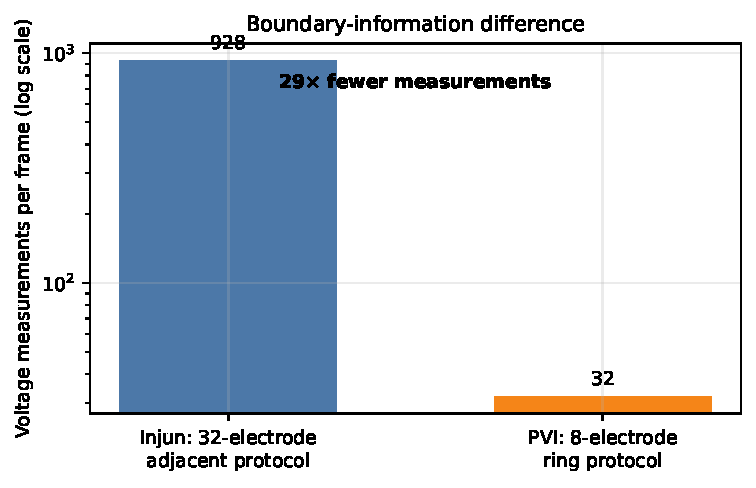
\includegraphics[width=0.72\linewidth]{measurement_comparison.pdf}
\caption{The original adjacent 32-electrode protocol supplies 928 scalar voltage
measurements per frame, whereas the PVI ring supplies 32.  This information deficit
is fundamental and cannot be removed by network capacity.}
\label{fig:measurement-count}
\end{figure}

\subsection{Notation}

\begin{longtable}{@{}p{0.18\linewidth}p{0.74\linewidth}@{}}
\caption{Notation used throughout the report.}\label{tab:notation}\\
\toprule
Symbol & Meaning \\
\midrule
\endfirsthead
\toprule
Symbol & Meaning \\
\midrule
\endhead
$\Omega\subset\R^2$ & Cross-sectional conductive domain. \\
$\sigma(\bm{x})$ & Conductivity field, in siemens per metre. \\
$u(\bm{x})$ & Interior electric potential. \\
$e_\ell$ & Boundary surface of electrode $\ell$. \\
$I_\ell,U_\ell,z_\ell$ & Electrode current, voltage, and contact impedance. \\
$\sig\in\R^K$ & Elementwise FEM conductivity vector. \\
$\bm{v}=F(\sig)\in\R^M$ & Nonlinear forward map from conductivity to measurements. \\
$J(\sig)\in\R^{M\times K}$ & Jacobian $\partial F/\partial\sig$. \\
$R$ & Spatial regularization operator or projected Laplacian. \\
$G=(\mathcal V,\mathcal E)$ & Graph whose nodes are FEM elements. \\
$\sig_k,\delta\sig_k$ & Conductivity estimate and LM update at stage $k$. \\
$\sig^*$ & Clean conductivity ground truth. \\
$\sig_b,\dsig$ & Baseline conductivity and time-varying conductivity change. \\
\bottomrule
\end{longtable}

\section{From telecommunications field theory to EIT}

\subsection{Quasi-static derivation}

At PVI frequencies and length scales, electromagnetic wave propagation is
negligible compared with conduction; the electric field is well approximated as
curl-free:
\begin{equation}
  \nabla\times\bm{E}=\bm{0},
  \qquad \bm{E}=-\nabla u.
\end{equation}
Ohm's constitutive relation is
\begin{equation}
  \bm{J}=\sigma\bm{E}=-\sigma\nabla u.
\end{equation}
Charge conservation in the absence of interior sources gives
\begin{equation}
  \nabla\cdot\bm{J}=0.
\end{equation}
Combining the three equations yields the EIT field equation
\begin{equation}
  \boxed{\nabla\cdot\left(\sigma\nabla u\right)=0\quad\text{in }\Omega.}
  \label{eq:eit-pde}
\end{equation}

\plain{The voltage distribution is not transmitted through the tissue as an
independent signal channel.  It is the solution of a boundary-value problem whose
coefficients are the unknown conductivity.  Changing conductivity changes all
measured boundary voltages in a spatially distributed way.}

\subsection{Complete electrode model}

Point-electrode models neglect contact impedance and finite electrode area.  The
PVI solver uses the complete electrode model (CEM).  For electrode $e_\ell$,
\begin{subequations}\label{eq:cem}
\begin{align}
  u + z_\ell\sigma\frac{\partial u}{\partial n} &= U_\ell
      &&\text{on }e_\ell,\\
  \int_{e_\ell}\sigma\frac{\partial u}{\partial n}\,\mathrm ds &= I_\ell,\\
  \sigma\frac{\partial u}{\partial n} &=0
      &&\text{outside the electrodes},\\
  \sum_{\ell=1}^{L} I_\ell &=0,
  \qquad \sum_{\ell=1}^{L} U_\ell=0.
\end{align}
\end{subequations}
The last voltage constraint fixes the arbitrary potential reference.

\subsection{Weak form and finite-element system}

Multiplying \cref{eq:eit-pde} by a test function $w$, integrating by parts, and
including the CEM terms produces the bilinear form
\begin{equation}
\begin{split}
  a_\sigma\big((u,\bm U),(w,\bm W)\big)
  =&\int_\Omega \sigma\nabla u\cdot\nabla w\,\mathrm d\bm x\\
  &+\sum_{\ell=1}^{L}\frac{1}{z_\ell}
  \int_{e_\ell}(u-U_\ell)(w-W_\ell)\,\mathrm ds,
\end{split}
\end{equation}
with right-hand side $\sum_\ell I_\ell W_\ell$.  Expanding $u$ in FEM basis
functions converts the problem into
\begin{equation}
  A(\sig)\bm\phi=\bm b,
  \qquad \bm v=M\bm\phi,
  \label{eq:fem-forward}
\end{equation}
where $A(\sig)$ is the conductivity-dependent stiffness/CEM matrix, $\bm\phi$
contains nodal and electrode potentials, and $M$ implements differential
measurements.

\section{The inverse problem}

\subsection{Measurement model}

The measured vector is
\begin{equation}
  \bm y = F(\sig^*) + \bm\varepsilon,
  \qquad \bm\varepsilon\sim \mathcal N(\bm0,\Sigma_\varepsilon)
  \label{eq:measurement-model}
\end{equation}
in the ideal Gaussian model.  A regularized estimate solves
\begin{equation}
  \widehat\sig = \operatorname*{arg\,min}_{\sig}
  \frac12\norm{\Sigma_\varepsilon^{-1/2}(F(\sig)-\bm y)}_2^2
  + \lambda^2\mathcal R(\sig).
  \label{eq:variational-inverse}
\end{equation}
For a quadratic spatial prior,
\begin{equation}
  \mathcal R(\sig)=\frac12\norm{R(\sig-\sig_{\mathrm{ref}})}_2^2.
\end{equation}

From a Bayesian perspective, the first term is the negative log likelihood and
the regularizer is the negative log prior.  The minimizer is a maximum a
posteriori estimate under those assumptions \cite{kaipio2005,lionheart2004}.

\subsection{Why the PVI inverse is severely underdetermined}

The local linearized system has $M=32$ measurements and $K=1330$ element values:
\begin{equation}
  J\in\R^{32\times1330},
  \qquad \operatorname{rank}(J)\le 32.
\end{equation}
Consequently,
\begin{equation}
  \dim\ker(J)\ge 1330-32=1298.
  \label{eq:nullity}
\end{equation}
At least 1,298 independent element directions are locally invisible to the data.
Regularization or learned priors select one solution among many data-consistent
fields; they do not create new physical information.

\plain{A clear-looking image is not automatically a correct image.  With only 32
measurements, a network can learn plausible vessel shapes that the voltages do not
uniquely support.  Independent nonlinear simulation, physical phantoms, and
uncertainty analysis are therefore mandatory.}

\section{Newton and Levenberg--Marquardt reconstruction}

\subsection{Linearization}

Around $\sig_k$, use the first-order Taylor approximation
\begin{equation}
  F(\sig_k+\bm p)\approx F(\sig_k)+J_k\bm p,
  \qquad J_k=J(\sig_k).
\end{equation}
Let $\bm r_k=F(\sig_k)-\bm y$ and $W=\Sigma_\varepsilon^{-1/2}$.  The quadratic
subproblem is
\begin{equation}
  \min_{\bm p}\frac12\norm{W(J_k\bm p+\bm r_k)}_2^2
  +\frac{\lambda^2}{2}\norm{R(\sig_k+\bm p-\sig_{\mathrm{ref}})}_2^2.
\end{equation}
Differentiating and setting the gradient to zero gives
\begin{equation}
\begin{split}
  &(J_k\trans W\trans WJ_k+\lambda^2R\trans R)\bm p_k\\
  &\quad=-J_k\trans W\trans W\bm r_k
  -\lambda^2R\trans R(\sig_k-\sig_{\mathrm{ref}}).
  \label{eq:gn-normal}
\end{split}
\end{equation}
Levenberg--Marquardt often replaces or augments the prior Hessian with
$\lambda I$, stabilizing weakly observed directions \cite{levenberg1944,marquardt1963}.

\subsection{Original code update}

Injun's code computes a normalized PyEIT Jacobian and uses
\begin{equation}
  \delta\sig_k=-\left(J_k\trans J_k+0.1I\right)^{-1}J_k\trans
  \left(F(\sig_k)-\bm y\right).
  \label{eq:original-lm}
\end{equation}
The update is not simply added to the current conductivity.  Instead,
$[\sig_k,\delta\sig_k]$ becomes the GCN input.

\subsection{Production PVI one-step inverse}

The strict MATLAB PVI path computes an unweighted coarse-mesh Jacobian $J_0$ at
$\sig_0=0.7\bm1$ and the projected fine-mesh Laplacian
\begin{equation}
  R_{\mathrm{rec}}=\frac12 C_{2F}\trans R_{\mathrm{fwd}}C_{2F}.
\end{equation}
Its fixed inverse matrix is
\begin{equation}
  D_1=(J_0\trans J_0+\lambda^2R_{\mathrm{rec}})^{-1}J_0\trans,
  \qquad \lambda=5\times10^{-4}.
\end{equation}
After reference subtraction, the historical displayed PVI convention is
\begin{equation}
  \dsig_{\mathrm{PVI}}=-D_1(\bm v_t-\bm v_0).
  \label{eq:pvi-display}
\end{equation}
Finite-difference tests show that the Python FEM Jacobian is the physical derivative
$\partial\bm v/\partial\sig$.  For clean physical conductivity supervision we
therefore use the sign-correct feature
\begin{equation}
  \dsig_{\mathrm{Newton}}=+D_1\dv.
  \label{eq:physical-newton}
\end{equation}

\section{Graph convolution as a learned spatial prior}

Let $A_G$ be the element-adjacency matrix.  With self-loops,
$\widetilde A=A_G+I$ and degree matrix $\widetilde D$, a standard GCN layer is
\begin{equation}
  H^{(\ell+1)}=phi\left(
  \widetilde D^{-1/2}\widetilde A\widetilde D^{-1/2}
  H^{(\ell)}W^{(\ell)}+\bm b^{(\ell)}
  \right).
  \label{eq:gcn}
\end{equation}
Neighbor aggregation acts like a learned, feature-dependent graph filter
\cite{kipf2017,fey2019}.  Unlike a fixed Laplacian penalty, nonlinear layers can
learn to preserve inclusion boundaries, reject isolated noise, and use patterns
that recur in the training distribution.

In an unrolled-optimization interpretation, the GCN approximates a learned
regularization or proximal map:
\begin{equation}
  \sig_{k+1}=\mathcal G_{\theta_k}
  \left(\sig_k,\delta\sig_k;G\right).
  \label{eq:learned-update}
\end{equation}
Each stage has different parameters because the error distribution evolves with
$k$.

\section{Injun Lee's original implementation: step by step}

The source audited here is \path{GCNM_training.py} and
\path{GCNM_testing.py}.  The workspace contains code but no saved original-run
metrics; this report records the experiment as specified and does not fabricate
numerical results.

\subsection{Original data experiment}

\begin{enumerate}[label=\textbf{O\arabic*.},leftmargin=2.5em]
\item Create 32-electrode circle or thorax forward/inverse PyEIT meshes.
\item Create the adjacent protocol: 32 excitations and 29 retained voltage
measurements per excitation, or 928 total.
\item Draw 500 phantoms with one to four non-overlapping ellipses.
\item Draw background conductivity in $[0.40,0.43]$, low inclusions in
$[0.15,0.25]$, and high inclusions in $[0.65,0.95]$.
\item Rasterize identical ellipse geometry onto fine and coarse meshes.
\item Simulate fine-mesh voltage and add Gaussian noise with standard scale
$0.005\operatorname{mean}|V|$.
\item Construct a graph in which inverse elements sharing any vertex are adjacent.
\end{enumerate}

\subsection{Original greedy GCNM training}

Initialize $\sig_0=\bm1$.  For $k=0,\ldots,9$:
\begin{enumerate}[label=\textbf{G\arabic*.},leftmargin=2.5em]
\item For every sample, set the inverse mesh to the current GCN estimate $\sig_k$.
\item Recompute $F(\sig_k)$ and normalized $J_k$.
\item Compute the LM feature using \cref{eq:original-lm}.
\item Set two node features $H_k=[\sig_k,\delta\sig_k]$.
\item Initialize a new GCN with widths $2\to250\to250\to250\to1$.
\item Train the GCN to predict the complete absolute $\sig^*$ using plain MSE.
\item Use an 80/20 ordered split, Adam at $0.002$, batch size 10, up to 10,000
epochs, and early-stopping patience 200.
\item Apply the best model to all samples; its direct output becomes $\sig_{k+1}$.
\item Save a separate checkpoint for stage $k$.
\end{enumerate}

The essential point is that the GCN does not output a step length or correction;
it directly predicts the next full conductivity.  The physics update is a feature.

\subsection{Original testing}

The test script creates 100 new synthetic samples from the same distribution.
Starting from $\sig_0=\bm1$, it recomputes the nonlinear LM update, loads GCN stage
$k$, predicts $\sig_{k+1}$, and repeats.  It reports relative conductivity
$\ell_1$ error, conductivity MSE, and forward-voltage relative $\ell_2$ error.
The root test script does not include a complete iterative-LM-only control, although
our modular extracted port later added one.

\begin{figure}[H]
\centering
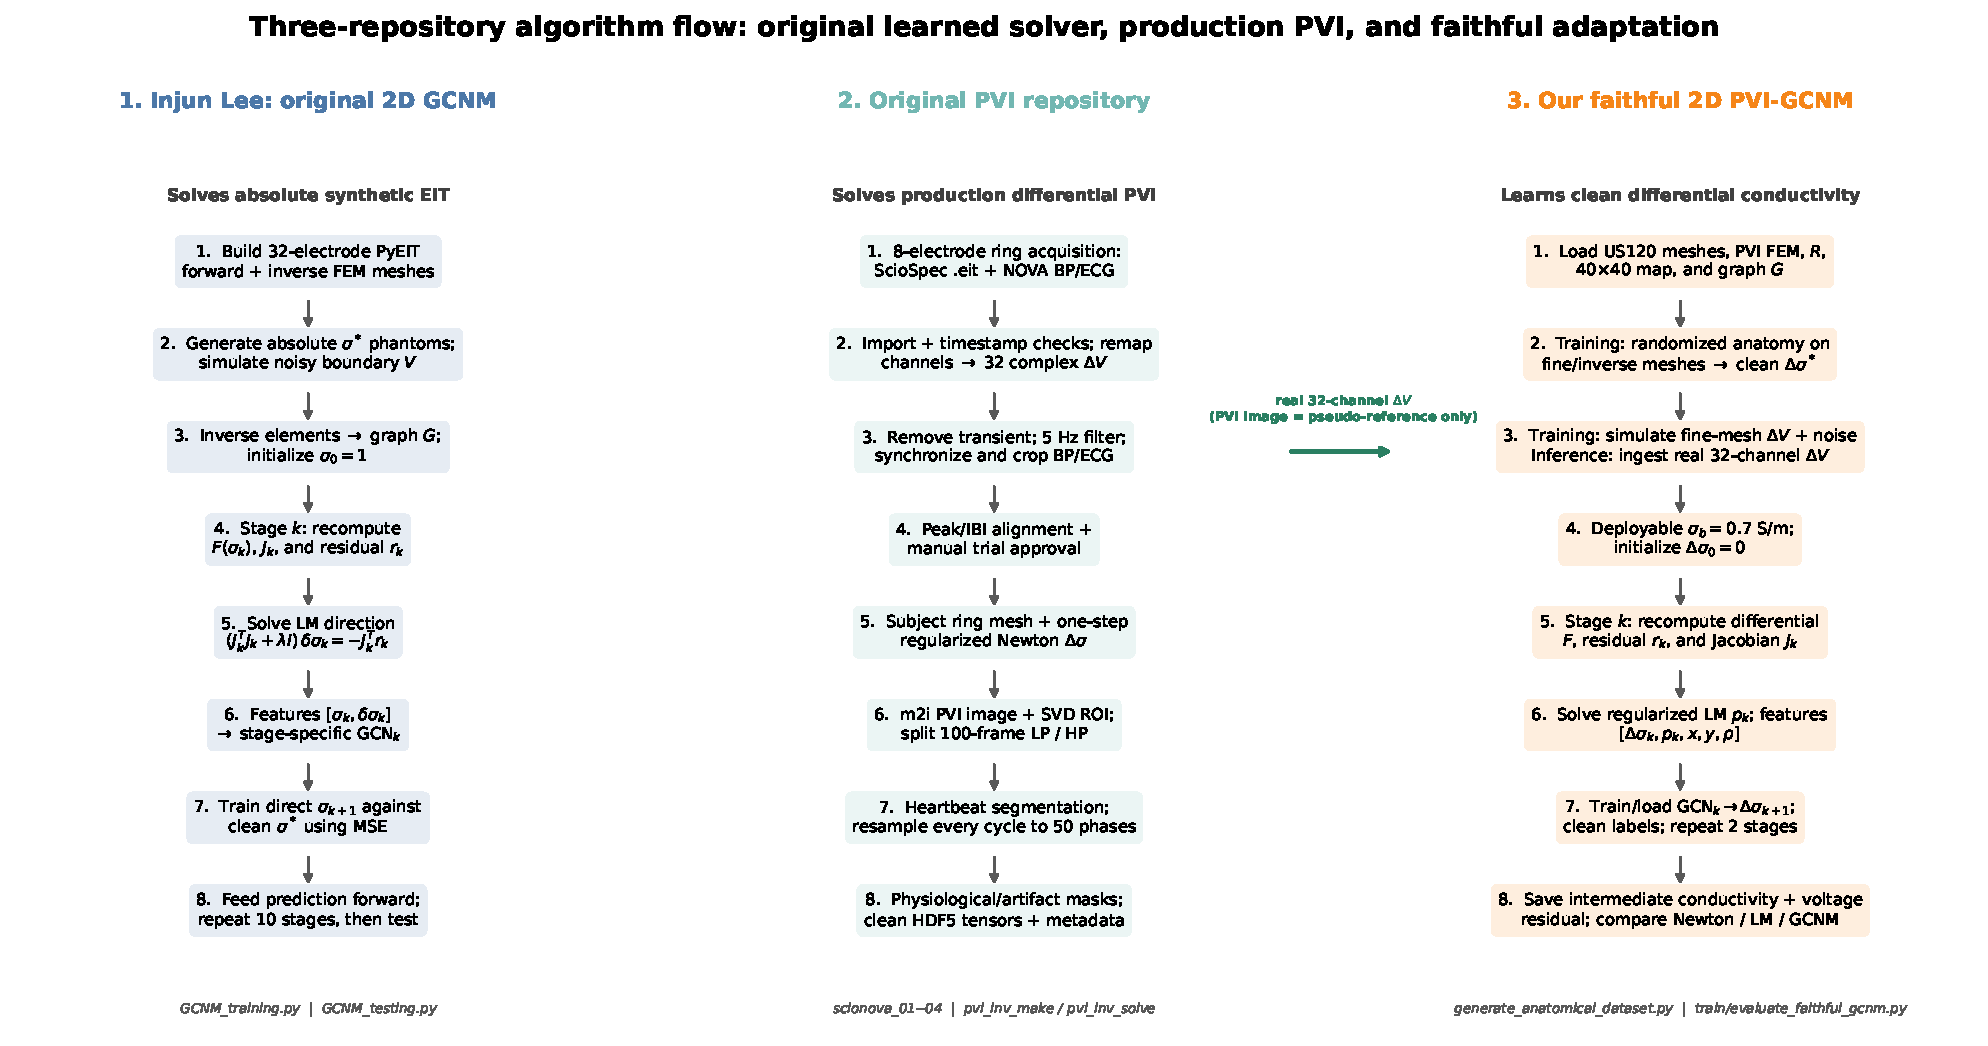
\includegraphics[width=0.98\linewidth]{algorithm_flow.pdf}
\caption{Step-by-step flow across the three repositories.  Left: Injun Lee's
original 32-electrode absolute-EIT GCNM.  Center: the eight-electrode production
PVI acquisition, reconstruction, cardiac segmentation, and export pipeline.
Right: our faithful differential PVI-GCNM, which combines clean simulated
conductivity supervision with newly recomputed PVI physics at every learned
stage.  The green cross-lane arrow is important: the PVI repository supplies real
32-channel voltage differences to our inference path; its Newton image is retained
only as a pseudo-reference, not as a clean label.}
\label{fig:algorithm-flow}
\end{figure}

\section{Our PVI adaptation}

\subsection{Production-parity foundation}

Before training a learned inverse, we reproduced the subject-6 production chain:
raw ScioSpec extraction, electrode remapping, signed 10-mA current, 5-Hz filtering,
resistance/reactance conversion, centered-shrink moving average, US120 geometry,
projected Laplacian, and MATLAB pixel ordering.  This separates two questions:
\begin{enumerate}
\item Is the input and deterministic inverse reproduced correctly?
\item Does a learned method improve reconstruction relative to that baseline?
\end{enumerate}

\subsection{Clean anatomical targets}

PVI images are not scientific labels in the anatomical experiment.  We generate
skin, fat, muscle, bone, blood, and one or two pulsatile vessels.  A shared
parameterization is rasterized independently on the 5,320-element forward mesh and
1,330-element inverse mesh.  The target is clean vascular $\dsig^*$.

The training generator has two modes:
\begin{align}
  \text{linearized: }&\quad \dv \approx J_{\mathrm{fine},q}\dsig^*_{\mathrm{fine}},\\
  \text{nonlinear: }&\quad \dv = F_{\mathrm{fine}}(\sig_b+\dsig^*)-F_{\mathrm{fine}}(\sig_b).
\end{align}
The linearized mode uses a bank of randomized anatomical fine-mesh Jacobians for
efficient training.  The exact nonlinear mode performs two separate FEM solves and
is reserved for an independent holdout.

Domain randomization includes static contact impedance, contact drift in nonlinear
simulation, channel gain, current gain, white noise, correlated noise, tissue
conductivity, layer thickness, bone geometry, vessel position, vessel axes, and
cardiac-phase amplitude.

\subsection{Earlier fixed-feature residual GCN}

The earlier model normalizes conductivity by the 99.5th training percentile $s$ and
uses five features:
\begin{equation}
  H_i=\left[\frac{\dsig_{k,i}}{s},\frac{n_i}{s},x_i,y_i,r_i\right],
  \qquad n=D_1\dv.
\end{equation}
It uses widths $5\to64\to64\to64\to1$.  The output is residual around Newton:
\begin{equation}
  \widehat{\dsig}_{k+1}=n+s\,g_{\theta_k}(H,G).
  \label{eq:our-residual}
\end{equation}
The final graph layer is initialized to zero, so the initial network exactly equals
Newton.

Because vessels occupy few elements, the training objective is weighted:
\begin{align}
  w_i &= 1+\alpha\operatorname{clip}
  \left(\frac{|y_i|}{\operatorname{median}_{j:y_j\ne0}|y_j|},0,2\right),\\
  \mathcal L &= \frac{1}{SK}\sum_{s=1}^{S}\sum_{i=1}^{K}
  w_{s,i}(\widehat y_{s,i}-y_{s,i})^2,
  \qquad \alpha=8.
  \label{eq:weighted-loss}
\end{align}
Two greedy stages were trained, but both reused $n$.  This is the principal
departure from the original method.

\begin{table}[H]
\centering
\caption{Methodological comparison.}
\label{tab:method-comparison}
\small
\begin{tabular}{@{}p{0.23\linewidth}p{0.34\linewidth}p{0.34\linewidth}@{}}
\toprule
Aspect & Injun original & Earlier fixed-feature PVI experiment \\
\midrule
Physics & PyEIT absolute forward problem & PVI CEM differential problem \\
Target & Absolute $\sig^*$ & Vascular $\dsig^*$ \\
Initial estimate & $\sig_0=\bm1$ & $\dsig_0=\bm0$ \\
Update per stage & New $F(\sig_k),J_k,\delta\sig_k$ & Fixed $n=D_1\dv$ reused \\
Features & $[\sig_k,\delta\sig_k]$ & $[\dsig_k,n,x,y,r]$ \\
Output & Direct full conductivity & Newton plus learned residual \\
Stages & 10 & 2 \\
Hidden widths & $250,250,250$ & $64,64,64$ \\
Loss & Unweighted MSE & Vessel-weighted MSE \\
Coordinates & No explicit coordinates & Explicit $x,y,r$ \\
Data & Generic ellipses & Randomized anatomy and vessels \\
Main control & Synthetic truth & Newton, linearized and nonlinear truth \\
\bottomrule
\end{tabular}
\end{table}

\subsection{Implemented faithful nonlinear PVI-GCNM}
\label{sec:faithful-implementation}

For a fixed inference baseline $\sig_b$ and current differential estimate
$\dsig_k$, the implemented stage predicts a differential voltage and forms
\begin{equation}
  \widehat{\dv}_k=F(\sig_b+\dsig_k)-F(\sig_b),
  \qquad \bm r_k=\widehat{\dv}_k-\dv_{\mathrm{meas}}.
  \label{eq:implemented-residual}
\end{equation}
The PVI solver recomputes $J_k=J(\sig_b+\dsig_k)$ and solves
\begin{equation}
  \left(J_k\trans J_k+h_{\mathrm{PVI}}^2R_{\mathrm{rec}}
  +\lambda_{\mathrm{LM}}I\right)\bm p_k
  =-J_k\trans\bm r_k.
  \label{eq:implemented-lm}
\end{equation}
Here $R_{\mathrm{rec}}$ is the projected inverse-mesh regularizer,
$h_{\mathrm{PVI}}$ preserves the production inverse scale, and the separate
$\lambda_{\mathrm{LM}}I$ stabilizes each stage-dependent solve.  The graph input
always contains $[\dsig_k,\bm p_k]$; the coordinate ablation adds $[x,y,r]$.

Two output parameterizations were executed:
\begin{align}
  \text{direct:}\quad &\dsig_{k+1}=g_{\theta_k}([\dsig_k,\bm p_k],G),\\
  \text{proposal residual:}\quad &\dsig_{k+1}=\dsig_k+\bm p_k
  +c_{\theta_k}([\dsig_k,\bm p_k],G).
\end{align}
The residual correction layer is zero initialized, and both modes project the
absolute conductivity $\sig_b+\dsig_{k+1}$ above a positive numerical floor.
A separate iterative-LM control applies exactly the same recomputed physics without
a GCN.  Training and inference bind the baseline policy, physics hyperparameters,
mesh, mappings, configuration, and dataset hashes in each checkpoint so an oracle
synthetic baseline cannot be silently used on real data.

\section{Experiments performed}

\subsection{E0: original code experiment specification}

The original code defines 500 training and 100 testing phantoms, ten greedy GCN
stages, and a $250^3$ hidden architecture.  No original-run result file is present
in this workspace.  Consequently, the original configuration is used as a method
reference, not as a numerical comparator.

\subsection{E1: production reconstruction parity}

Using 500 frame-matched subject-6 HDF samples, reconstructed high-pass images were
compared directly with the archived MATLAB output.

\begin{table}[H]
\centering
\caption{Production-parity experiment.  This validates the port, not learned image quality.}
\label{tab:parity}
\begin{tabular}{@{}lr@{}}
\toprule
Metric & Value \\
\midrule
Frames & 500 \\
Finite pixels & 1,364 \\
Finite-mask IoU & 1.0000 \\
Global image correlation & 0.9936 \\
Median per-frame correlation & 0.9914 \\
Minimum per-frame correlation & 0.9776 \\
Image RMSE & $6.86\times10^{-4}$ \\
Normalized RMSE & 0.1131 \\
Optimal scale & 0.9907 \\
\bottomrule
\end{tabular}
\end{table}

\subsection{E2: temporal alignment and engineering pseudo-label packs}

Automatic segmentation produced 1,310 candidates; 1,298 were monotonically matched
to the HDF sequence across 11 trials.  Low-pass resistance and reactance mean-channel
correlations were 0.99982 and 0.99999.  High-pass correlations were lower
(approximately 0.67) because archived manual peak merges were unavailable.

A leakage-controlled engineering pack retained 971 clean periods and ten phases
per period: 6,930 train samples from trials 1--7, 1,180 validation samples from
trials 8--9, and 1,600 test samples from trials 10--11.  These labels reproduce
PVI and are suitable only for pipeline testing, not superiority claims.

\subsection{E3: earlier fixed-feature clean-truth experiment}

The full clean experiment used 512 training, 128 validation, and 128 test samples.
Each split used eight independently randomized fine-mesh Jacobian backgrounds.
Training used two stages, $64^3$ hidden widths, batch size 16, learning rate
$10^{-3}$, 150 requested epochs, patience 15, and $\alpha=8$ vessel weighting.

\subsection{E4: exact nonlinear holdout}

Thirty-two independent test phantoms were generated by separate baseline and
dynamic fine-mesh FEM solves.  They were never used for training or checkpoint
selection.  This is the stronger distribution-shift test because neither the
linearized data approximation nor the training Jacobian bank creates their voltage.

\subsection{E5: faithful core and physical control}

The faithful core trained two stage-specific GCNs while recomputing
\cref{eq:implemented-residual,eq:implemented-lm} at each stage.  Controlled pairs
used direct versus proposal-residual output, and the same forward/Jacobian code ran
two LM iterations with no learning.  A saved-anatomy synthetic baseline was retained
only as an oracle upper bound.  Every deployable experiment trained and inferred
with the same homogeneous $0.7$~S/m baseline.

\subsection{E6: controlled architecture and objective ablations}

Starting from the homogeneous direct core, experiments added mesh coordinates,
swept vessel weights $\alpha\in\{0,1,2,4,8\}$, and then swept explicit background
penalties $\beta\in\{0.25,0.5,1.0\}$ at the selected $\alpha=1$.  The background
runs selected checkpoints with a composite normalized-RMSE/background/Dice score.
Only one factor changed in each comparison, every experiment used seed 0, and model
and result directories were isolated to prevent checkpoint overwrites.

\subsection{Compute execution}

The production chain, smoke tests, faithful core, and all synthetic ablations
completed with exit code \texttt{0:0} and empty error logs.  Every training and
evaluation launcher preserved the requested allocation: one node, one task, one
GPU, 16 CPUs, 250~GB, and a one-day wall-time limit on the \texttt{ece\_bst}
partition and account.

\begin{table}[H]
\centering
\caption{Executed Slurm experiment groups.  Ranges include training and dependent
linearized, nonlinear, or real-PVI evaluations as applicable.}
\label{tab:slurm}
\begin{tabular}{@{}lll@{}}
\toprule
Jobs & Purpose & State \\
\midrule
426833--426837 & Earlier fixed-feature data, training, and evaluation & completed \\
426840--426844 & Faithful end-to-end smoke and voltage-sign verification & completed \\
426893--426900 & Homogeneous direct/residual core and real controls & completed \\
426901--426915 & Coordinates and $\alpha$ sweeps & completed \\
426921--426929 & Background-penalty sweep & completed \\
426938 & Selected-model full real-PVI evaluation & completed \\
\bottomrule
\end{tabular}
\end{table}

\begin{figure}[H]
\centering
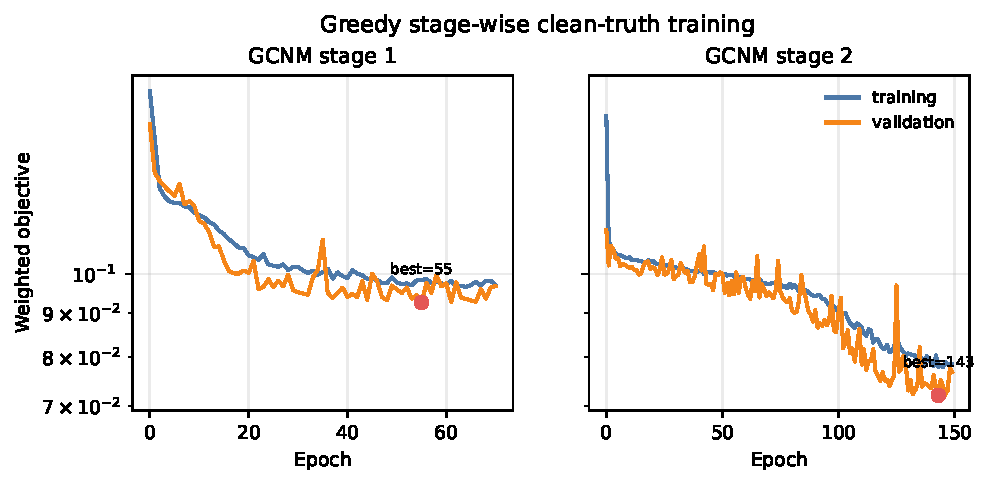
\includegraphics[width=0.94\linewidth]{training_curves.pdf}
\caption{Greedy weighted-objective training.  Stage 1 reached its best validation
objective around epoch 55; stage 2 continued to approximately epoch 143.  Lower
weighted loss does not guarantee lower unweighted background RMSE.}
\label{fig:training-curves}
\end{figure}

\section{Quantitative results}

\subsection{Historical fixed-feature linearized holdout}

\begin{table}[H]
\centering
\caption{Results on 128 independently generated linearized holdout samples.}
\label{tab:linearized-results}
\begin{tabular}{@{}lrrr@{}}
\toprule
Metric & Newton & GCNM stage 1 & GCNM stage 2 \\
\midrule
Element correlation $\uparrow$ & 0.129 & 0.329 & \textbf{0.420} \\
Image correlation $\uparrow$ & 0.209 & 0.339 & \textbf{0.435} \\
Localization Dice $\uparrow$ & 0.239 & 0.357 & \textbf{0.433} \\
Element RMSE $\downarrow$ & \textbf{0.00457} & 0.00712 & 0.00674 \\
Image RMSE $\downarrow$ & \textbf{0.00613} & 0.01134 & 0.01072 \\
Background RMS $\downarrow$ & \textbf{0.00251} & 0.00684 & 0.00653 \\
\bottomrule
\end{tabular}
\end{table}

GCNM finds more correct spatial support, but overestimates structure and background.
Stage 2 partially corrects stage-1 amplitude while further improving localization.

\subsection{Historical fixed-feature exact nonlinear holdout}

\begin{table}[H]
\centering
\caption{Results on 32 exact nonlinear fine-mesh holdout samples.}
\label{tab:nonlinear-results}
\begin{tabular}{@{}lrrr@{}}
\toprule
Metric & Newton & GCNM stage 1 & GCNM stage 2 \\
\midrule
Element correlation $\uparrow$ & 0.175 & 0.373 & \textbf{0.445} \\
Image correlation $\uparrow$ & 0.265 & 0.388 & \textbf{0.463} \\
Localization Dice $\uparrow$ & 0.295 & 0.307 & \textbf{0.359} \\
Element RMSE $\downarrow$ & 0.00354 & \textbf{0.00345} & 0.00365 \\
Image RMSE $\downarrow$ & 0.00506 & \textbf{0.00502} & 0.00541 \\
Background RMS $\downarrow$ & \textbf{0.00063} & 0.00202 & 0.00281 \\
\bottomrule
\end{tabular}
\end{table}

Stage 1 is the best balanced estimator: compared with Newton, it more than doubles
element correlation, increases image correlation from 0.265 to 0.388, and slightly
reduces both element and image RMSE.  Stage 2 obtains the best localization and
correlation but loses RMSE performance.

\begin{figure}[H]
\centering
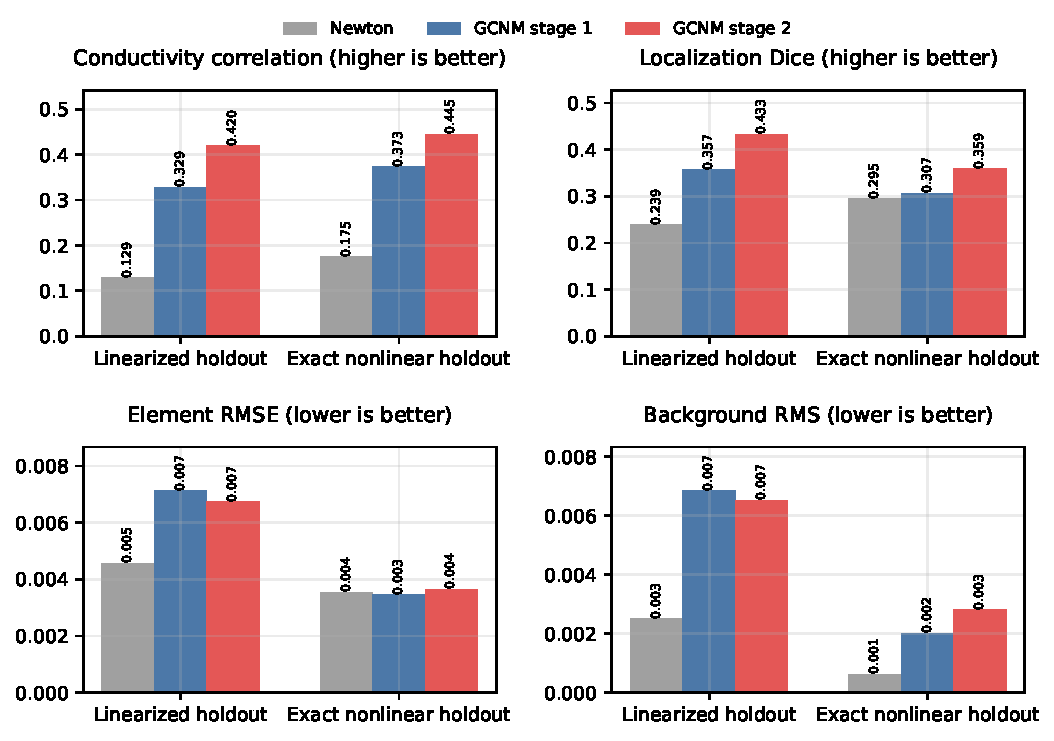
\includegraphics[width=0.98\linewidth]{stage_results.pdf}
\caption{Stage-wise clean-truth metrics.  The result is a Pareto trade-off: GCNM
improves structure-sensitive metrics but increases false background energy.}
\label{fig:stage-results}
\end{figure}

\subsection{Faithful core and iterative-physics control}

The matched core comparison in \cref{tab:faithful-core} uses the same 32 exact
nonlinear phantoms.  Merely repeating the nonlinear LM solve improves Dice more
than the historical saved Newton step but only modestly improves correlation.
Learning supplies a larger structural gain.  Direct output is stronger than the
proposal-residual parameterization on correlation, RMSE, and Dice, so direct output
was retained for subsequent ablations.

\begin{table}[H]
\centering
\caption{Faithful homogeneous-baseline core on the exact nonlinear holdout.
Voltage RMS is the physical residual after stage 2; a dash means it was not recorded
for that historical artifact.}
\label{tab:faithful-core}
\small
\resizebox{\linewidth}{!}{%
\begin{tabular}{@{}lrrrrr@{}}
\toprule
Method & Image corr. $\uparrow$ & Image RMSE $\downarrow$ & Dice $\uparrow$ & BG RMS $\downarrow$ & Voltage RMS $\downarrow$ \\
\midrule
Historical saved Newton & 0.265 & 0.00506 & 0.295 & 0.000626 & -- \\
Iterative LM, stage 2 & 0.291 & 0.00503 & \textbf{0.394} & 0.000589 & \textbf{$1.90\times10^{-7}$} \\
Earlier fixed-feature GCN, stage 2 & \textbf{0.463} & 0.00541 & 0.359 & 0.002810 & -- \\
Faithful direct, stage 2 & 0.458 & \textbf{0.00484} & 0.230 & 0.000581 & $2.73\times10^{-6}$ \\
Faithful proposal-residual, stage 2 & 0.390 & 0.00494 & 0.176 & \textbf{0.000474} & $1.36\times10^{-6}$ \\
\bottomrule
\end{tabular}}
\end{table}

\begin{figure}[H]
\centering
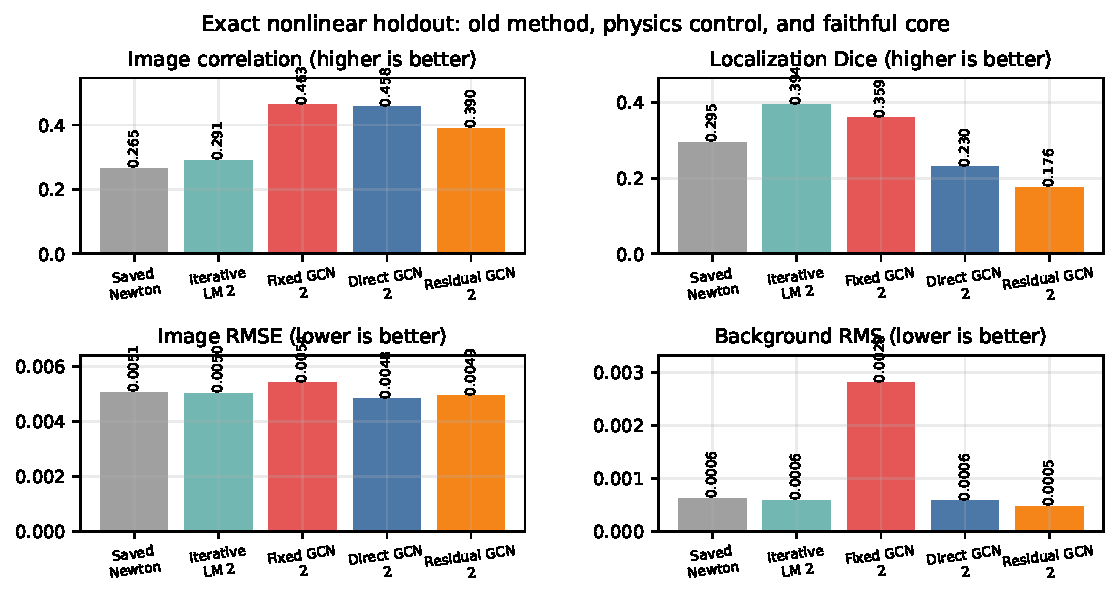
\includegraphics[width=0.98\linewidth]{faithful_core_comparison.pdf}
\caption{Historical Newton and fixed-feature results, iterative-LM-only control,
and the two implemented faithful output parameterizations.  No single bar should
be read alone: structure, amplitude, localization, and background expose different
failure modes.}
\label{fig:faithful-core}
\end{figure}

\subsection{Baseline knowledge is an oracle ablation}

The saved synthetic $\sig_b$ contains static vessel locations.  It is therefore
information unavailable during deployment, not an acceptable default input.  It
raises direct-core correlation from 0.458 to 0.520, demonstrating that baseline
knowledge matters, but all remaining models use the homogeneous $0.7$~S/m policy.

\begin{table}[H]
\centering
\caption{Baseline-policy ablation for faithful direct output.}
\label{tab:baseline-ablation}
\begin{tabular}{@{}lrrrr@{}}
\toprule
Baseline & Image corr. $\uparrow$ & RMSE $\downarrow$ & Dice $\uparrow$ & BG RMS $\downarrow$ \\
\midrule
Saved anatomy (oracle only) & 0.520 & \textbf{0.00456} & \textbf{0.346} & 0.000737 \\
Homogeneous 0.7 S/m (deployable) & 0.458 & 0.00484 & 0.230 & \textbf{0.000581} \\
\bottomrule
\end{tabular}
\end{table}

\begin{figure}[H]
\centering
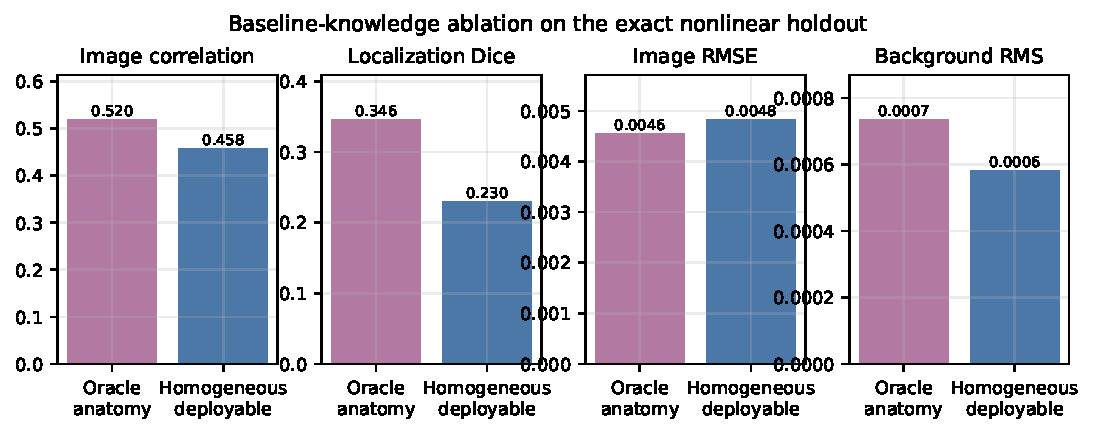
\includegraphics[width=0.98\linewidth]{faithful_baseline_comparison.pdf}
\caption{Explicit oracle-versus-deployable baseline comparison.  The oracle result
must not be quoted as real-data performance.}
\label{fig:faithful-baseline}
\end{figure}

\subsection{Architecture and loss ablations}

Coordinates provide the largest isolated architectural improvement.  Vessel
weighting $\alpha=1$ maximizes Dice and minimizes RMSE but also increases false
background and voltage mismatch.  A background coefficient of 0.25 recovers nearly
the same correlation with lower background; larger coefficients continue suppressing
background but erase vessel support.  We therefore select the balanced
$\alpha=1,\beta=0.25$ model rather than optimizing any single metric.

\begin{table}[H]
\centering
\caption{Deployable homogeneous-baseline stage-2 ablations on 32 exact nonlinear
holdout samples.  ``Mean corr.'' is the mean of per-sample image correlations;
``global corr.'' pools all valid pixels.}
\label{tab:faithful-ablation}
\scriptsize
\resizebox{\linewidth}{!}{%
\begin{tabular}{@{}lrrrrrr@{}}
\toprule
Experiment & Global corr. $\uparrow$ & Mean corr. $\uparrow$ & RMSE $\downarrow$ & Dice $\uparrow$ & BG RMS $\downarrow$ & Voltage RMS $\downarrow$ \\
\midrule
Direct core & 0.458 & 0.419 & 0.00484 & 0.230 & \textbf{0.000581} & $2.73\times10^{-6}$ \\
Proposal residual & 0.390 & 0.331 & 0.00494 & 0.176 & 0.000474 & $1.36\times10^{-6}$ \\
Direct + coordinates & \textbf{0.561} & 0.545 & 0.00444 & 0.471 & 0.000865 & $1.73\times10^{-6}$ \\
$\alpha=1$ & 0.557 & \textbf{0.581} & \textbf{0.00430} & \textbf{0.543} & 0.001541 & $4.62\times10^{-6}$ \\
$\alpha=2$ & 0.524 & 0.507 & 0.00445 & 0.457 & 0.001778 & $5.93\times10^{-6}$ \\
$\alpha=4$ & 0.489 & 0.468 & 0.00477 & 0.407 & 0.002232 & $7.32\times10^{-6}$ \\
$\alpha=8$ & 0.479 & 0.454 & 0.00519 & 0.394 & 0.002730 & $1.02\times10^{-5}$ \\
$\alpha=1,\beta=0.25$ (selected) & 0.557 & 0.567 & 0.00432 & 0.485 & 0.001276 & $3.18\times10^{-6}$ \\
$\alpha=1,\beta=0.5$ & 0.530 & 0.492 & 0.00446 & 0.462 & 0.000992 & $1.87\times10^{-6}$ \\
$\alpha=1,\beta=1.0$ & 0.527 & 0.469 & 0.00453 & 0.427 & 0.000845 & \textbf{$1.58\times10^{-6}$} \\
\bottomrule
\end{tabular}}
\end{table}

\begin{figure}[H]
\centering
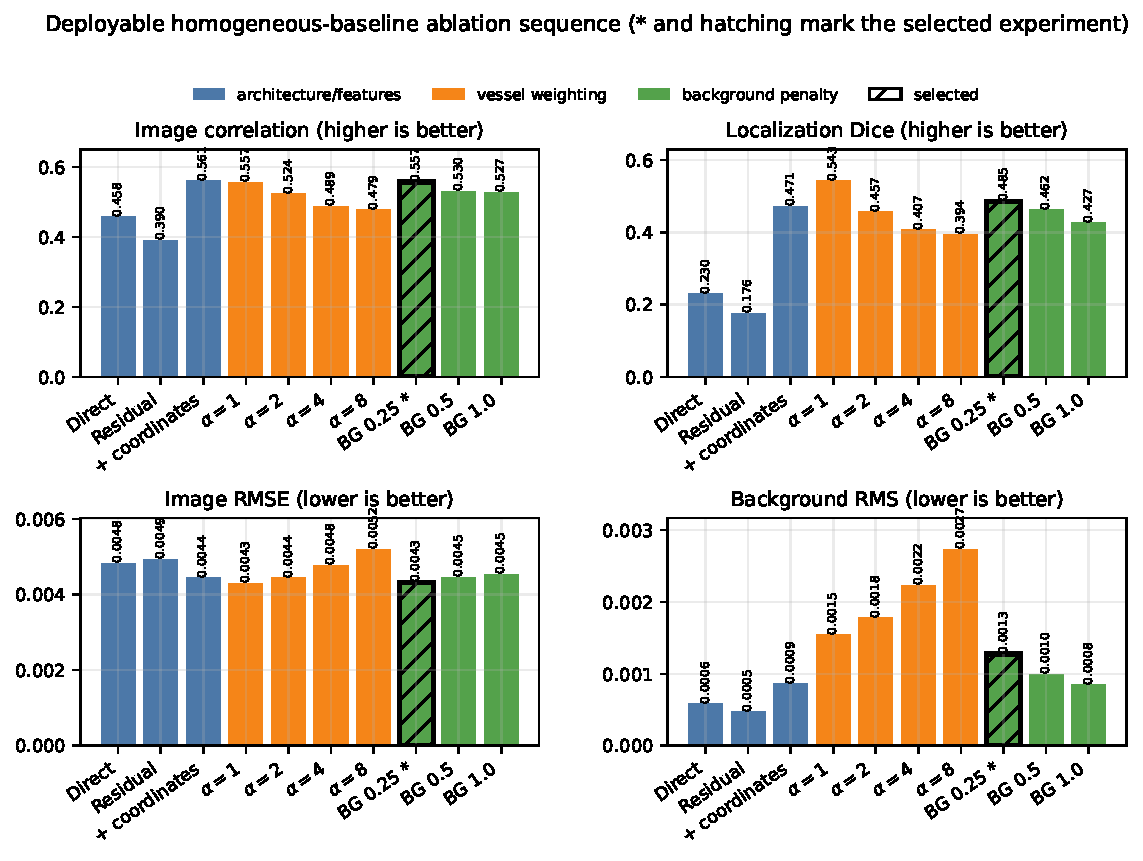
\includegraphics[width=0.98\linewidth]{faithful_ablation_comparison.pdf}
\caption{Complete deployable ablation sequence.  The selected background-0.25
model is marked in the generated figure.}
\label{fig:faithful-ablation}
\end{figure}

\section{Qualitative output comparisons}

Numerical averages answer whether an estimator improves on a population, but they
do not show \emph{how} it fails.  This section therefore compares conductivity maps
with fixed spatial registration and matched color scales.  It separates three
questions that must not be conflated:
\begin{enumerate}[label=(\roman*)]
\item did the earlier fixed-feature clean-truth experiment improve over its smoke run;
\item how close were those earlier predictions to known synthetic ground truth; and
\item how do the earlier outputs compare with real PVI reconstructions, for which
      anatomical conductivity ground truth is unavailable?
\end{enumerate}

\subsection{Smoke versus earlier fixed-feature experiment on an identical phantom}

The anatomical smoke evaluation and sample 0 of the earlier exact nonlinear
holdout contain the \emph{same} clean conductivity target and the same Newton input
to floating-point precision.  This permits a direct experiment-evolution comparison.
The previous model used one stage with only three training and one validation sample;
the fixed-feature model used two stages with 512 training and 128 validation samples.

\begin{figure}[H]
\centering
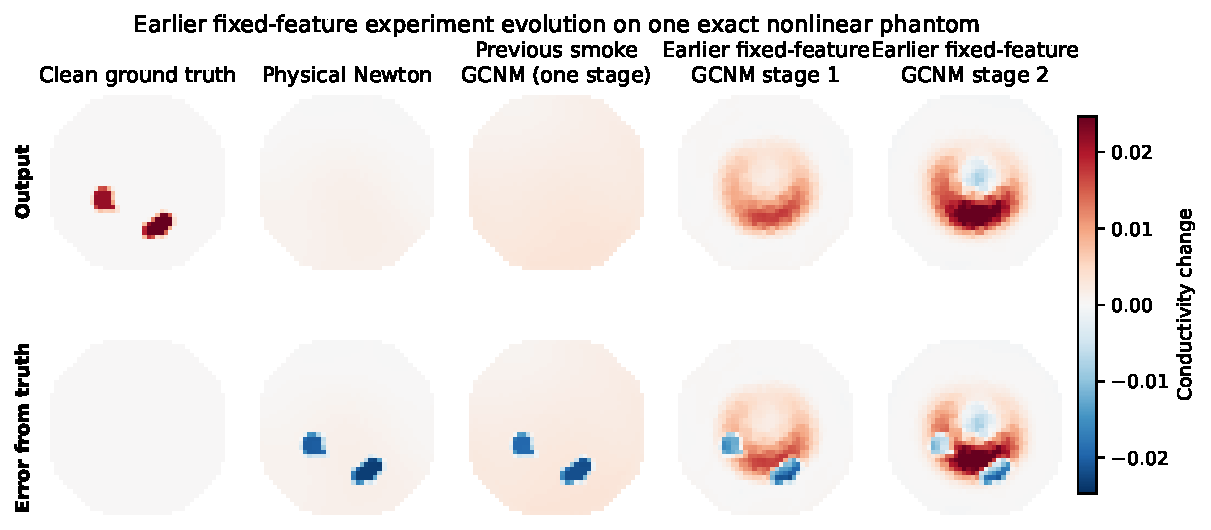
\includegraphics[width=\linewidth]{experiment_evolution.pdf}
\caption{Direct output evolution on the same exact nonlinear phantom.  The top row
shows reconstructed conductivity change; the bottom row is prediction minus clean
ground truth.  The previous smoke GCN is nearly a spatially uniform bias.  The fixed-feature
models recover the broad vessel-bearing region, but not the two compact vessel
boundaries; stage 2 additionally creates a central negative artifact.}
\label{fig:experiment-evolution}
\end{figure}

\begin{table}[H]
\centering
\caption{Pixel-matched metrics for the single shared phantom in
\cref{fig:experiment-evolution}.  This controlled example shows algorithm evolution,
not population performance; the 32-sample averages remain in
\cref{tab:nonlinear-results}.}
\label{tab:shared-sample-results}
\begin{tabular}{@{}lrrrr@{}}
\toprule
Method & Image corr. $\uparrow$ & Element RMSE $\downarrow$ & BG-RMS $\downarrow$ & Dice $\uparrow$ \\
\midrule
Newton & 0.258 & \textbf{0.00296} & \textbf{0.00075} & \textbf{0.455} \\
Previous smoke GCN & 0.182 & 0.00343 & 0.00215 & 0.000 \\
Fixed-feature GCN stage 1 & 0.317 & 0.00323 & 0.00247 & 0.091 \\
Fixed-feature GCN stage 2 & \textbf{0.319} & 0.00430 & 0.00400 & 0.136 \\
\bottomrule
\end{tabular}
\end{table}

The fixed-feature method is clearly more structured than the smoke model, but this example
also demonstrates why image appearance or correlation alone is insufficient.  The
learned stages improve image correlation while worsening RMSE, background energy, and
Dice relative to Newton on this particular phantom.  The diffuse arc has roughly the
correct global location but not the correct vessel support.

\subsection{Ground truth versus earlier fixed-feature predictions}

To avoid selecting only a visually favorable example,
\cref{fig:clean-truth-gallery} selects the best, median, and worst stage-2 cases by
image correlation among all 32 exact nonlinear samples.  The selected sample indices
are 30, 26, and 21 with correlations 0.641, 0.423, and 0.147, respectively.  Each row
uses one shared conductivity scale, so amplitude and background errors remain visible.

\begin{figure}[H]
\centering
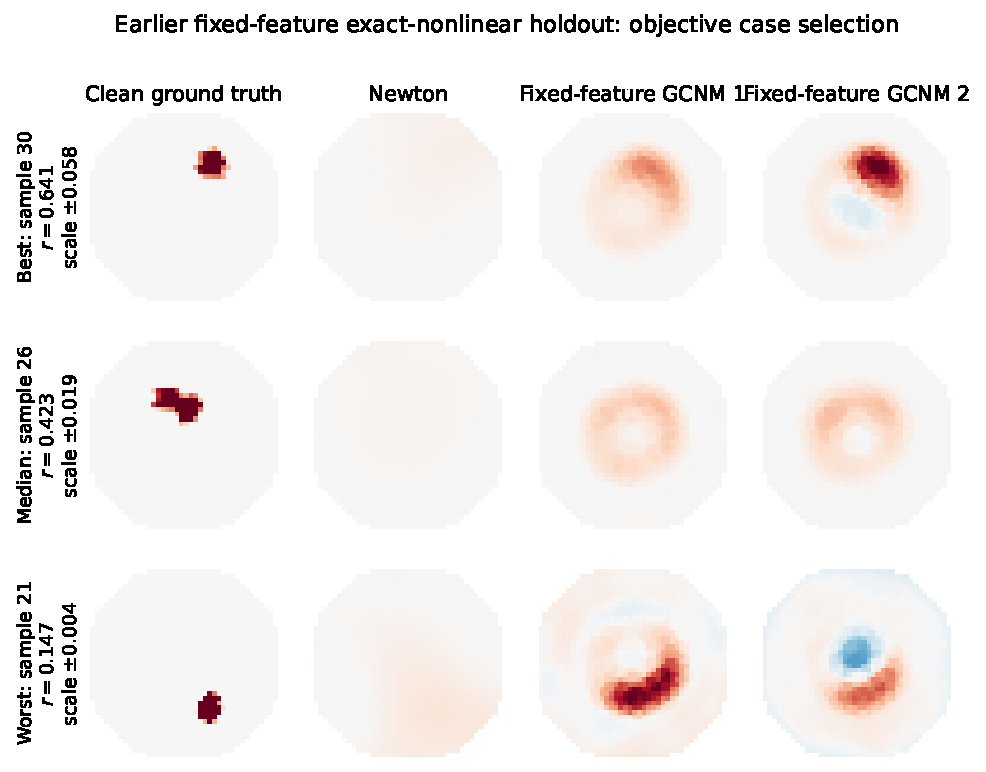
\includegraphics[width=\linewidth,height=0.68\textheight,keepaspectratio]{clean_truth_gallery.pdf}
\caption{Clean ground truth, physical Newton reconstruction, and the two earlier fixed-feature GCN
stages for objectively selected nonlinear-holdout cases.  GCNM usually moves energy
toward the correct region, but predicts a smooth distribution learned from the
anatomical prior rather than resolving the compact ground-truth vessels.  The worst
case also shows sign-changing background structure.}
\label{fig:clean-truth-gallery}
\end{figure}

\subsection{Selected faithful model versus ground truth and prior outputs}

The selected faithful gallery repeats the best/median/worst protocol using final
stage image correlation over all 32 nonlinear holdout samples.  Every row includes
the clean target, historical saved Newton, iterative LM control, earlier fixed
feature GCN, and both faithful stages.  This is the most direct visual answer to
whether recomputed physics and the controlled ablations improved the intermediate
conductivity representation.

\begin{figure}[H]
\centering
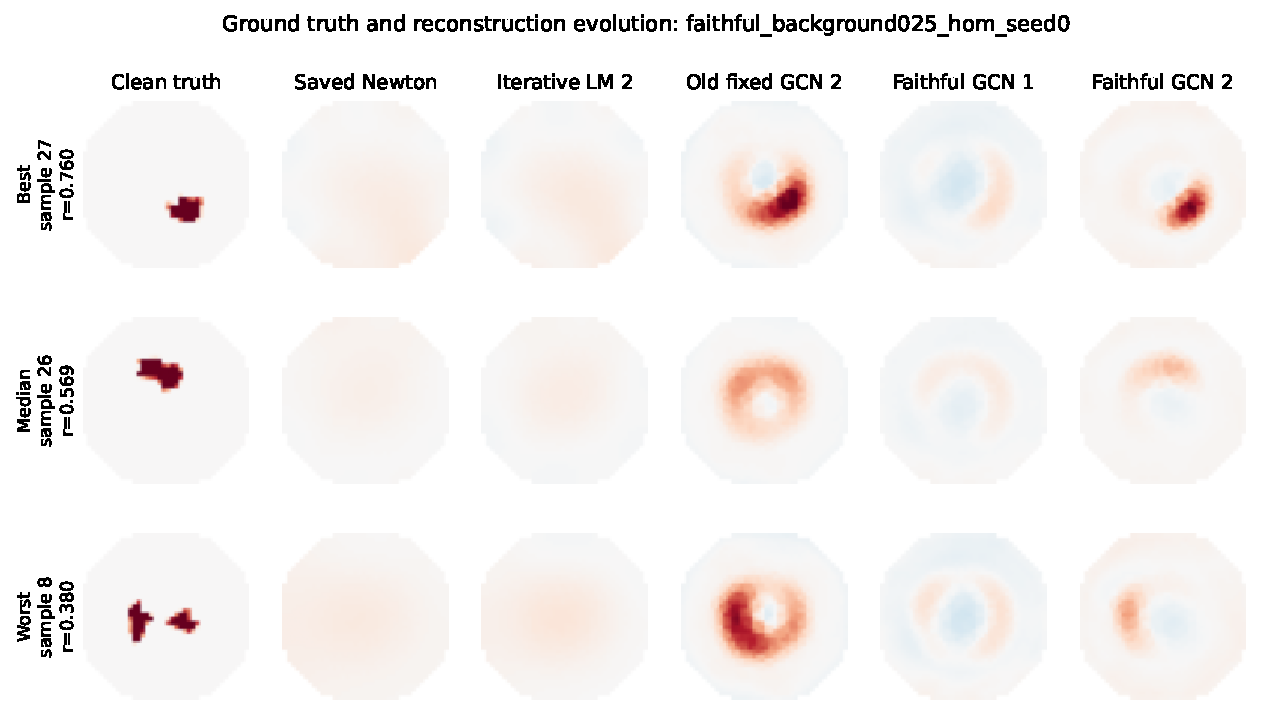
\includegraphics[width=\linewidth]{faithful_output_gallery.pdf}
\caption{Clean ground truth and reconstruction evolution for the selected
$\alpha=1,\beta=0.25$ homogeneous-baseline model.  Rows are selected objectively
as best, median, and worst final-stage image correlation; the color scale is shared
within each row.}
\label{fig:faithful-output-gallery}
\end{figure}

\subsection{Comparison with archived PVI images}

The real PVI images have no paired anatomical conductivity truth.  They are themselves
regularized one-step Newton reconstructions produced by the MATLAB pipeline.  Thus,
the only valid pixelwise question is whether our production port and earlier GCN
reproduce those images---not whether either image is anatomically correct.

\begin{figure}[H]
\centering
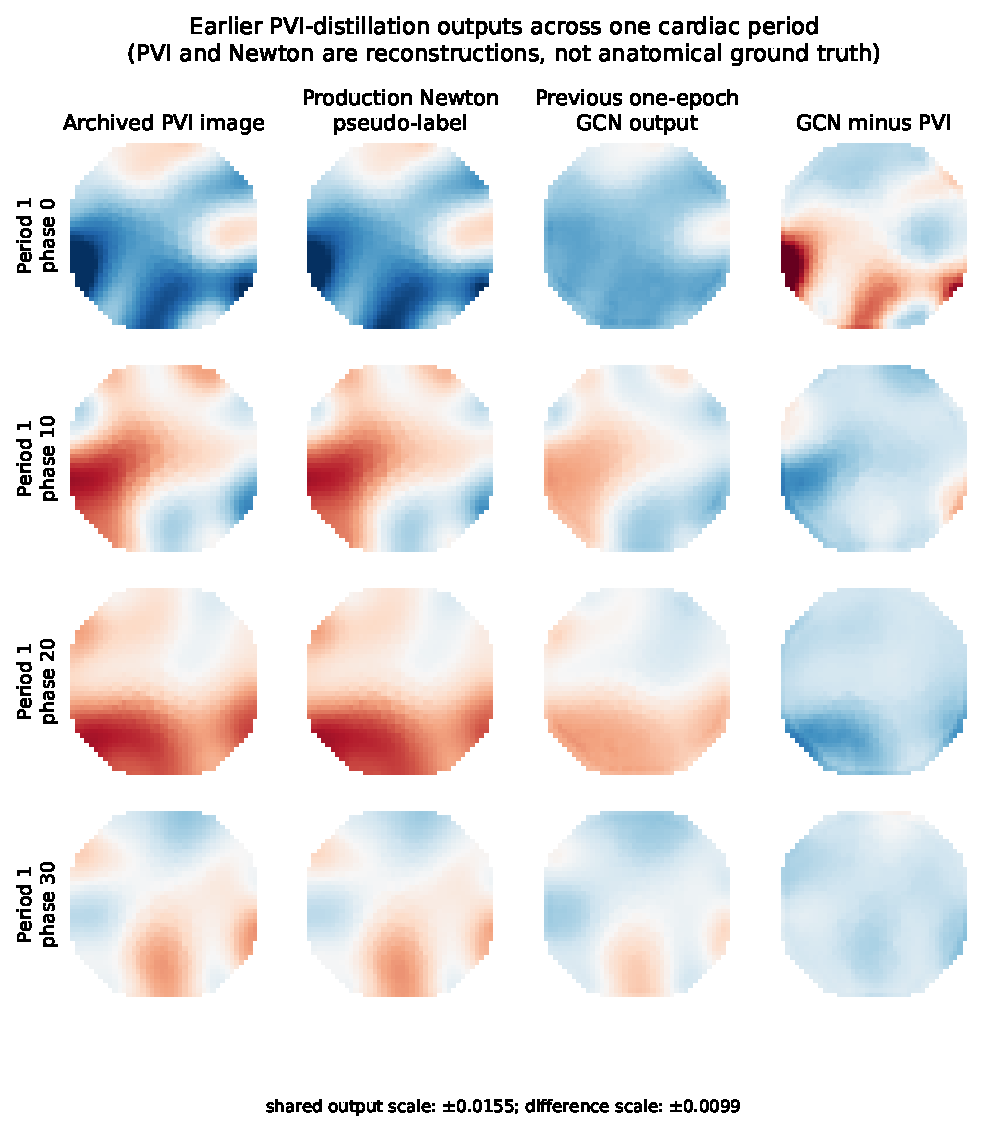
\includegraphics[height=0.72\textheight,keepaspectratio]{pvi_output_comparison.pdf}
\caption{Four phases from subject 6, period 1.  Columns compare the archived MATLAB
PVI image, our production Newton pseudo-label, and the earlier one-epoch GCN output;
the final column is GCN minus archived PVI.  The first two columns agree closely,
whereas the GCN attenuates and smooths the image.  These displayed examples belong
to the ten-sample smoke train/validation pack and are descriptive, not independent
test evidence.}
\label{fig:pvi-output-comparison}
\end{figure}

\begin{table}[H]
\centering
\caption{Meaning of the real-PVI comparisons.  Correlation with PVI measures
reproduction of the existing inverse, not anatomical recovery.}
\label{tab:pvi-visual-metrics}
\small
\begin{tabular}{@{}L{5.0cm}rrL{4.0cm}@{}}
\toprule
Comparison & Samples & Image corr. & Interpretation \\
\midrule
Production pseudo-label vs. archived PVI & 10 & 0.9929 & MATLAB/Python inverse parity \\
Previous GCN vs. archived PVI & 10 & 0.9628 & Smoke train/validation imitation \\
Previous GCN vs. production pseudo-label & 10 & 0.9715 & Distillation fit, not clean truth \\
Previous GCN vs. pseudo-label, held-out trials & 4 & 0.9828 & Independent trials 10--11, but the label is still PVI Newton \\
\bottomrule
\end{tabular}
\end{table}

The final faithful model was also evaluated on all 1,600 test phases from trials
10--11.  The iterative-LM panels below are reused from the shared homogeneous-core
evaluation, while the faithful panels are produced by the selected background-0.25
checkpoint.  The reference is deliberately labeled ``pseudo-reference'': agreement
or disagreement quantifies relation to the existing PVI inverse, never anatomical
correctness.

\begin{figure}[H]
\centering
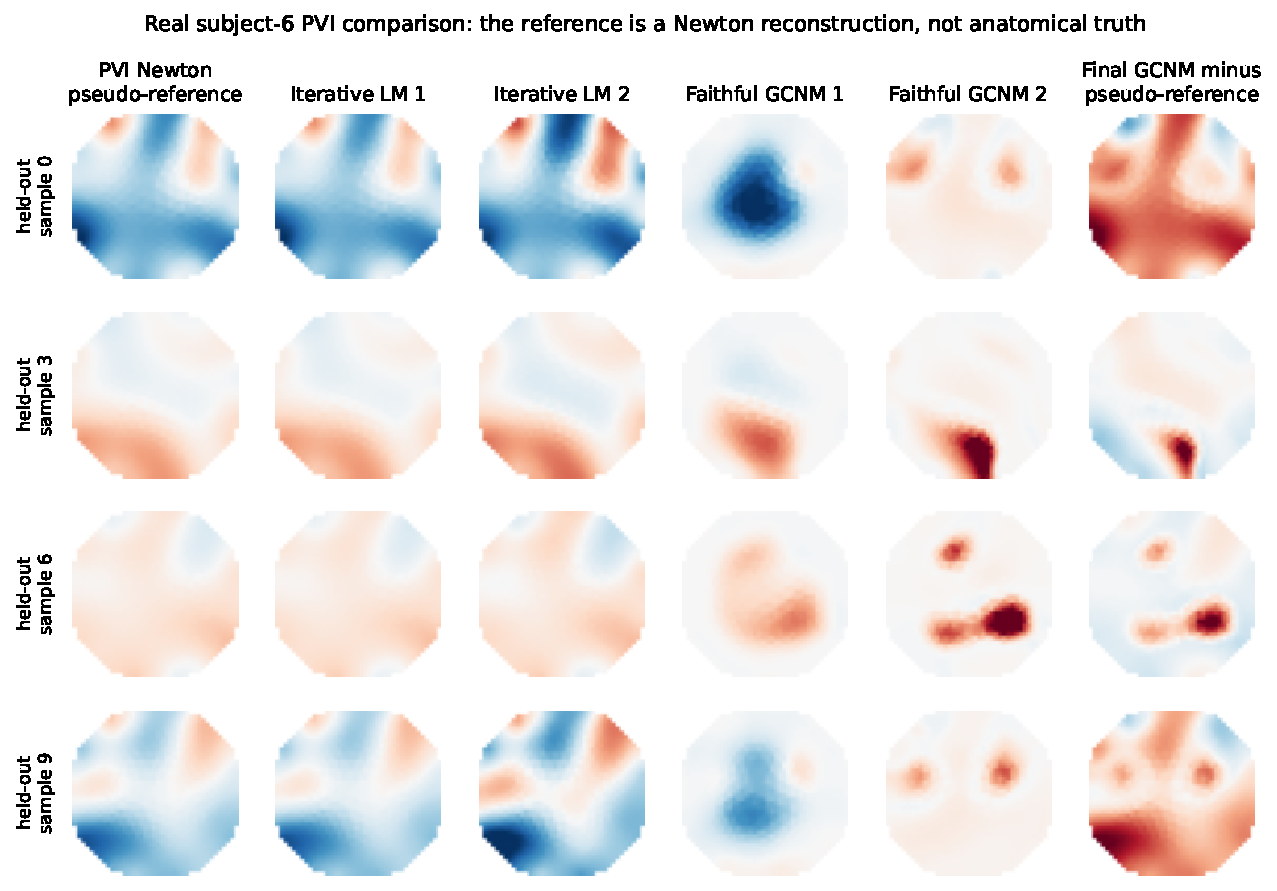
\includegraphics[width=\linewidth]{faithful_real_pvi_gallery.pdf}
\caption{Full-test real subject-6 comparison for deterministic held-out phases.
The PVI Newton pseudo-reference, two iterative-LM stages, two selected faithful
GCNM stages, and final difference map are registered on the same inverse mesh.
No synthetic Dice or vessel-ground-truth claim is transferred to this panel.}
\label{fig:faithful-real-pvi}
\end{figure}

\begin{table}[H]
\centering
\caption{Full 1,600-phase real-PVI pseudo-reference comparison.  Correlation and
RMSE are relative to the production Newton image, not anatomical truth.  The first
LM step reproduces that reference by construction.}
\label{tab:faithful-real-pvi}
\scriptsize
\resizebox{\linewidth}{!}{%
\begin{tabular}{@{}lrrrr@{}}
\toprule
Method & Global image corr. & Mean per-sample corr. & Image RMSE & Post-stage voltage RMS \\
\midrule
Iterative LM stage 1 & 1.000 & 1.000 & $2.42\times10^{-10}$ & $6.66\times10^{-6}$ \\
Iterative LM stage 2 & 0.977 & 0.971 & 0.00279 & $5.98\times10^{-6}$ \\
Faithful direct stage 1 & 0.619 & 0.724 & 0.00821 & $2.00\times10^{-5}$ \\
Faithful direct stage 2 & 0.212 & 0.348 & 0.00921 & $2.06\times10^{-5}$ \\
Faithful proposal-residual stage 1 & 0.821 & 0.927 & 0.00686 & $1.79\times10^{-5}$ \\
Faithful proposal-residual stage 2 & 0.424 & 0.555 & 0.00826 & $2.00\times10^{-5}$ \\
Selected $\alpha=1,\beta=0.25$ stage 1 & 0.604 & 0.443 & 0.00713 & $1.68\times10^{-5}$ \\
Selected $\alpha=1,\beta=0.25$ stage 2 & 0.169 & 0.275 & 0.01059 & $2.63\times10^{-5}$ \\
\bottomrule
\end{tabular}}
\end{table}

The selected model reduces the physical voltage residual at stage 1 but stage 2
reverses that gain and departs further from the production inverse.  This is direct
evidence of synthetic-to-real distribution shift and a reason to expose intermediate
stages rather than only the final image.  It does not identify which image is more
anatomically correct; that decision requires an external reference.

\begin{table}[H]
\centering
\caption{Why the clean-truth and PVI panels must be read differently.}
\label{tab:supervision-semantics}
\begin{tabular}{@{}L{3.0cm}L{3.2cm}L{3.3cm}L{3.0cm}@{}}
\toprule
Panel & Target/reference & What can be concluded & What cannot be concluded \\
\midrule
Earlier and faithful anatomical & Known fine-mesh vessel conductivity & Localization and amplitude error against truth & Immediate visual realism on a human acquisition \\
Archived PVI & MATLAB Newton reconstruction & Port parity and temporal consistency & Anatomical correctness or vessel resolution \\
Previous PVI GCN & Same Newton image used as feature and label & Ability to imitate/compress the existing inverse & Improvement beyond Newton \\
Cross-domain visual comparison & Unpaired synthetic and real samples & Gross scale, smoothness, and artifact differences & Pixelwise accuracy or subject-specific anatomy \\
\bottomrule
\end{tabular}
\end{table}

\section{Interpretation at bachelor and doctoral levels}

\subsection{Why correlation improves while RMSE worsens}

Correlation is invariant to positive global scaling and rewards matching spatial
variation.  RMSE penalizes amplitude and background at every element.  A prediction
can therefore place high values near the correct vessel but remain too broad or too
large:
\begin{equation}
  \widehat\sig=a\sig^*+\bm b_{\mathrm{diffuse}},
  \quad a>1,
\end{equation}
yielding high correlation and poor RMSE.  The vessel-weighted objective in
\cref{eq:weighted-loss} explicitly makes this outcome more likely because missing a
vessel costs more than creating moderate background.

\subsection{Why the earlier stage 2 amplified background}

In the original algorithm, stage 2 is constrained by a new residual and Jacobian.
In the earlier fixed-feature experiment, both stages saw the same Newton feature
$n$.  Stage 2 could use the stage-1 image as context, but no new physical discrepancy
identified unsupported features.  Reapplying the learned prior therefore sharpened
localization while amplifying artifacts.  The faithful method fixes this
methodological defect by recomputing $\bm r_k$, $J_k$, and $\bm p_k$.  It does not,
however, guarantee monotone voltage descent: a learned direct output can still trade
data consistency for a conductivity prior, which is why voltage RMS remains an
explicit reported metric.

\subsection{Identifiability and learned hallucination}

Let the singular value decomposition be $J=U\Sigma V\trans$.  Only right singular
vectors with nonzero singular values are observed.  A learned network supplies
components in the approximate nullspace:
\begin{equation}
  \widehat\sig=J^\dagger\dv + (I-J^\dagger J)\,\mathcal P_\theta(\dv),
  \label{eq:nullspace-learning}
\end{equation}
where $\mathcal P_\theta$ is a learned prior.  The second term can improve a target
drawn from the same distribution, but it can also hallucinate under distribution
shift.  Equation \eqref{eq:nullspace-learning} is a useful conceptual decomposition,
not the literal network implementation.

\subsection{Why the original problem is easier}

The original protocol supplies 928 measurements, whereas PVI supplies 32.  Even
before considering noise and electrode mismatch, the PVI Fisher information
$J\trans\Sigma_\varepsilon^{-1}J$ has rank at most 32.  The original method also
trains and tests on generic ellipses from nearly the same simulator, while our
strongest test uses an exact nonlinear forward solve after training on a linearized
Jacobian bank.  Direct performance expectations must account for both differences.

\section{Implemented faithful solver and execution safeguards}

The faithful equations are implemented exactly as
\cref{eq:implemented-residual,eq:implemented-lm}; no unimplemented whitening
matrix or alternative normal equation is inserted in the report.  The real PVI
pack stores the MATLAB display-sign convention, so evaluation multiplies saved
voltages by $-1$ before physical inversion and records that sign in its JSON report.
Synthetic solver voltages use sign $+1$.

The deployable baseline is homogeneous $0.7$~S/m in training and inference.  The
saved-anatomy mode is explicitly named oracle, and checkpoint loading rejects an
incompatible baseline contract.  Configuration, mesh, mapping, and dataset hashes
make accidental cross-experiment reuse detectable.  Positivity projection counts
are reported at every stage; a zero count establishes that a run did not rely on
clipping, although it does not prove physiological validity.

\section{Executed ablations and remaining validation}

\subsection{Completed controlled sequence}

The faithful core, iterative-LM control, direct/residual output comparison,
coordinate ablation, vessel-weight sweep, background-penalty sweep, and composite
checkpoint selection were all executed.  The principal findings are:
\begin{enumerate}
\item recomputed LM physics alone improves Dice but cannot match learned spatial
correlation;
\item direct output outperforms proposal-residual output on clean reconstruction;
\item coordinates materially improve the eight-electrode inverse because the mesh
prior is strongly location dependent;
\item $\alpha=1$ is preferable to larger vessel weights, which progressively amplify
background and voltage inconsistency; and
\item $\beta=0.25$ is the balanced selected model, while $\beta=0.5$ and $1.0$
demonstrate the expected noise--localization Pareto frontier.
\end{enumerate}

\subsection{Scale and uncertainty}

Run at least five simulator seeds and report confidence intervals.  Increase the
number of independent anatomical Jacobian backgrounds.  Evaluate calibration by
ensembles or Monte Carlo dropout, and test whether uncertainty increases in
low-sensitivity/nullspace regions.

\subsection{Real-data validation hierarchy}

Recommended evidence, from strongest to weakest, is:
\begin{enumerate}
\item physical tank/limb phantom with known inclusion location and conductivity;
\item co-registered ultrasound or another independent vessel-location target;
\item held-out forward-voltage consistency with realistic electrode nuisance;
\item temporal repeatability and cardiac-phase coherence;
\item downstream blood-pressure prediction;
\item visual comparison with PVI images.
\end{enumerate}
The last item alone cannot establish anatomical validity because PVI is itself a
regularized reconstruction.

\section{Reproducibility map}

\begin{longtable}{@{}p{0.38\linewidth}p{0.53\linewidth}@{}}
\caption{Public implementation and reproducibility files.}\label{tab:files}\\
\toprule
Path & Role \\
\midrule
\endfirsthead
\toprule
Path & Role \\
\midrule
\endhead
\path{gcnm_pvi/gcnm_physics.py} & PVI forward/Jacobian and generic iterative LM interface. \\
\path{gcnm_pvi/iterative_physics.py} & Stage-dependent differential residual, Jacobian, LM proposal, and diagnostics. \\
\path{gcnm_pvi/gcnm_model.py} & Direct and proposal-residual graph blocks. \\
\path{gcnm_pvi/anatomical_phantoms.py} & Shared coarse/fine anatomical generator. \\
\path{gcnm_pvi/generate_anatomical_dataset.py} & Linearized-bank and exact nonlinear datasets. \\
\path{gcnm_pvi/train_faithful_gcnm.py} & Greedy faithful training, losses, checkpoint contract, and hashes. \\
\path{gcnm_pvi/evaluate_faithful_gcnm.py} & Newton, LM, faithful GCNM, voltage, and real-PVI evaluation. \\
\path{gcnm_pvi/summarize_faithful_results.py} & Cross-experiment metric summaries. \\
\path{configs/subject006_anatomical_gcnm.yaml} & Full clean experiment configuration. \\
\path{scripts/submit_faithful_experiment.sh} & Dependency-controlled training and evaluation submission. \\
\path{scripts/submit_faithful_weight_sweep.sh} & Coordinate and vessel-weight ablations. \\
\path{scripts/submit_faithful_background_sweep.sh} & Background-penalty ablations. \\
\path{slurm/launch_train_faithful.sh} & Fixed-resource cluster training entrypoint. \\
\path{slurm/launch_evaluate_faithful.sh} & Fixed-resource cluster evaluation entrypoint. \\
\path{tests/test_iterative_physics.py} & Physics sign, descent, and per-stage recomputation tests. \\
\path{tests/test_faithful_model.py} & Proposal-residual initialization test. \\
\path{reports/gcnm_pvi_latex/make_faithful_figures.py} & Static figures from private result artifacts. \\
\bottomrule
\end{longtable}

\section{Conclusions}

Injun Lee's original code is a greedy unrolled inverse solver: nonlinear physics is
recomputed, an LM update is formed, and a stage-specific GCN directly predicts the
next conductivity.  Our PVI work successfully replaced PyEIT with the PVI CEM
solver, resolved subject-6 US120 geometry, reproduced MATLAB production output,
created clean anatomical vascular supervision, introduced anti-inverse-crime
forward/inverse discretizations, and evaluated on an exact nonlinear holdout.

The project now contains and has executed the faithful nonlinear mechanism, not
only a proposal.  On the exact nonlinear holdout, two LM-only iterations reach
image correlation 0.291 and Dice 0.394.  The selected faithful homogeneous model
reaches correlation 0.557, RMSE 0.00432, Dice 0.485, and background RMS 0.00128.
It improves structural recovery substantially over saved Newton and the earlier
fixed-feature experiment while exposing a measurable trade-off between vessel
support, background suppression, and voltage consistency.

The correct conclusion is still not that eight-electrode GCNM has recovered true
human vascular anatomy.  The inverse has 32 measurements for 1,330 element unknowns,
and learned priors necessarily act in poorly observed subspaces.  The completed
real-PVI evaluation establishes execution, sign, temporal registration, and
pseudo-reference comparison only.  The next scientific evidence must come from
multiple simulator seeds and uncertainty intervals, more independent anatomical
backgrounds, a physical phantom, and co-registered ultrasound or another external
anatomical reference.

\appendix

\section{Pseudocode: original GCNM}

\begin{lstlisting}
Generate fine-mesh voltages V_s and coarse-mesh truths sigma*_s
Build FEM element graph G
Initialize sigma_0,s = 1 for every sample s

for k = 0,...,9:
    for each sample s:
        U_k,s, J_k,s = forward_and_normalized_jacobian(sigma_k,s)
        residual = U_k,s - V_s
        p_k,s = -(J^T J + lambda I)^(-1) J^T residual
        H_k,s = [sigma_k,s, p_k,s]

    train a new GCN_k to minimize mean ||GCN_k(H_k,s,G)-sigma*_s||^2
    sigma_k+1,s = GCN_k(H_k,s,G) for all samples
    save GCN_k
\end{lstlisting}

\section{Pseudocode: implemented faithful differential PVI-GCNM}

\begin{lstlisting}
Choose one baseline policy and bind it in every checkpoint
Generate measured differential voltage dV_s
Initialize dsigma_0,s = 0
Cache U_base,s = F(sigma_b,s)

for k = 0,...,K-1:
    for each sample s:
        U_k, J_k = forward_and_jacobian(sigma_b,s + dsigma_k,s)
        residual = (U_k - U_base) - dV_s
        p_k,s = solve(J^T J + h_pvi^2 Rrec + lambda_lm I,
                      -J^T residual)
        H_k,s = [dsigma_k,s, p_k,s]

    train a separate GCN_k against clean dsigma*_s
    direct mode:   dsigma_k+1,s = GCN_k(H_k,s,G)
    residual mode: dsigma_k+1,s = dsigma_k,s + p_k,s
                                  + correction_k(H_k,s,G)
    project sigma_b,s + dsigma_k+1,s above conductivity floor
    save GCN_k plus baseline, physics, configuration, and hashes
\end{lstlisting}

\section{Metric definitions}

For $S$ samples and $K$ elements,
\begin{align}
  \mathrm{RMSE} &= \sqrt{\frac{1}{SK}\sum_{s,i}
  (\widehat\sigma_{s,i}-\sigma^*_{s,i})^2},\\
  \mathrm{BG\mbox{-}RMS} &= \sqrt{
  \frac{\sum_{s,i}(1-m_{s,i})\widehat\sigma_{s,i}^2}
       {\sum_{s,i}(1-m_{s,i})}},\\
  \mathrm{Dice}_{\mathrm{volume}} &=
  \frac{2|\widehat{\mathcal S}\cap\mathcal S^*|}
       {|\widehat{\mathcal S}|+|\mathcal S^*|}.
\end{align}
Here $\mathcal S^*$ is the true nonzero support and $\widehat{\mathcal S}$ contains
the same number of elements with largest predicted magnitude.  Because the two
sets have equal size, the implemented Dice reduces numerically to
$|\widehat{\mathcal S}\cap\mathcal S^*|/|\mathcal S^*|$.

\begin{thebibliography}{9}

\bibitem{holder2005}
D. S. Holder, ed.,
\emph{Electrical Impedance Tomography: Methods, History and Applications},
Institute of Physics Publishing, 2005.

\bibitem{lionheart2004}
W. R. B. Lionheart,
``EIT reconstruction algorithms: pitfalls, challenges and recent developments,''
\emph{Physiological Measurement}, vol. 25, pp. 125--142, 2004.

\bibitem{kaipio2005}
J. Kaipio and E. Somersalo,
\emph{Statistical and Computational Inverse Problems},
Springer, 2005.

\bibitem{levenberg1944}
K. Levenberg,
``A method for the solution of certain non-linear problems in least squares,''
\emph{Quarterly of Applied Mathematics}, vol. 2, pp. 164--168, 1944.

\bibitem{marquardt1963}
D. W. Marquardt,
``An algorithm for least-squares estimation of nonlinear parameters,''
\emph{Journal of the Society for Industrial and Applied Mathematics},
vol. 11, no. 2, pp. 431--441, 1963.

\bibitem{kipf2017}
T. N. Kipf and M. Welling,
``Semi-supervised classification with graph convolutional networks,''
in \emph{International Conference on Learning Representations}, 2017.

\bibitem{fey2019}
M. Fey and J. E. Lenssen,
``Fast graph representation learning with PyTorch Geometric,''
in \emph{ICLR Workshop on Representation Learning on Graphs and Manifolds}, 2019.

\end{thebibliography}

\end{document}
